\documentclass[12pt,letterpaper]{article}
\usepackage[utf8]{inputenc}
\usepackage{amsmath}
\usepackage{amsfonts}
\usepackage{amssymb}
\usepackage{makeidx}
\usepackage{graphicx}
\usepackage[normalem]{ulem}
%\usepackage[doublespacing]{setspace}
\usepackage{subcaption}
\usepackage{float}
\usepackage{longtable}
\usepackage{titlesec}
\usepackage[margin=1in]{geometry}
\usepackage{ntheorem}
\usepackage{booktabs}
\usepackage{dcolumn}
\usepackage{adjustbox}
\usepackage[stable]{footmisc}
\usepackage{multirow}
\usepackage{tikz}
\usetikzlibrary{arrows,calc, patterns, positioning, shapes.geometric, decorations.pathreplacing,decorations.markings}
\usepackage{ntheorem}
\newtheorem{hyp}{Hypothesis} 
\newtheorem{subhyp}{Hypothesis}[hyp]
\renewcommand\thesubhyp{\thehyp.\alph{subhyp}}
\usepackage[round]{natbib}
\bibpunct{(}{)}{;}{a}{}{,~}
\usepackage[space]{grffile}
\usepackage[affil-it]{authblk}
\usepackage{epigraph}
\makeatletter

\def\@maketitle{%
	\newpage
	\null
	\vskip 2em%
	\begin{center}%
		\let \footnote \thanks
		{\Large\bfseries \@title \par}%
		\vskip 1.5em%
		{\normalsize
			\lineskip .5em%
			\begin{tabular}[t]{c}%
				\@author
			\end{tabular}\par}%
		{\normalsize \@date}%
	\end{center}%
	\par
	}
\makeatother

\title{After Deterrence: Explaining Conflict Short of War}

\author{J Andr\'{e}s Gannon%
	\thanks{Address correspondence to: \texttt{jagannon@ucsd.edu}}}
\affil{Department of Political Science \\ University of California, San Diego}

\author{Erik Gartzke%
	\thanks{Electronic address: \texttt{egartzke@ucsd.edu}}}
\affil{Department of Political Science\\ Director, Center for Peace and Security Studies (cPASS)\\ University of California, San Diego}

\author{Jon R. Lindsay%
	\thanks{Electronic address: \texttt{jon.lindsay@utoronto.ca} \\ The authors wish to thank the members of the Cross-Domain Deterrence Initiative, the Center for Peace and Security Studies (cPASS), and the Department of Defense Strategic Multi-layer Assessment for thoughtful feedback. Benjamin Smalley provided excellent research assistance. Earlier drafts of this paper were presented at the 10$^{th}$ Annual Strategic Multi-layer Assessment (SMA) Conference and the 2016 ISAC-ISSS Annual Conference. This research was sponsored by Office of Naval Research Grant N00014-14-1-0071 and the Department of Defense Minerva Research Initiative. Any opinions, findings, and conclusions or recommendations expressed in this publication are those of the authors and do not necessarily reflect the view of the Office of Naval Research.}}
\affil{Munk School of Global Affairs\\ University of Toronto}


\begin{document}

\maketitle

\begin{abstract}
	\noindent Policymakers are increasingly concerned about conflict ``in the gray zone" --- the region between peace and war where, it is feared, challengers are able to alter the status quo without fear of triggering a larger military confrontation. Paradigmatic examples include the Russian annexation of Crimea and incursion into Eastern Ukraine and China's island building campaign in the South China Sea. Here, we define gray zone conflict in a manner that emphasizes theoretical consistency and highlights novel features and implications of its causes. While gray zone conflicts are often perceived as deterrence failures, they are better understood as responses to deterrence success. A key puzzle involves understanding why capable countries choose to fight in a limited fashion. To the degree that gray zone conflict results from prior deterrence successes, raising the cost of limited war could yield peace. Alternatively, the decision to fight in the gray zone could reflect an optimal low-cost war fighting strategy, in which case doubling down on deterrence risks escalation and broader war.
\end{abstract}

\newpage

\setlength{\epigraphwidth}{4.5in}
\epigraph{That is not a Cold War. It is a grey war. Permanently teetering on the edge of outright hostility. Persistently hovering around the threshold of what we would normally consider acts of war.}{Sir Michael Fallon, former British Secretary of State for Defence}

\section{Introduction}
	In the wake of the overthrow of Ukrainian President Viktor Yanukovych in February 2014,  Russian special forces (``Spetsnaz'') and the 810\textsuperscript{th} Independent Naval Infantry Brigade occupied the Crimean Peninsula \citep{kofman_lessonsrussiaoperations_2017}. These forces had removed their military insignia, leading to initial speculation about their identity and whether or not their actions were sanctioned by the Kremlin. The undesignated Russian forces were accompanied by local police from the Berkut public order unit and were also joined by armed local self-defense volunteers. After the dust had settled, Russia's role in coordinating this invasion as well as their goals of taking over Crimea became abundantly clear. The action prompted considerable concern in NATO countries about how to counter a novel threat that did not quite meet formal thresholds for a coordinated military response, but which was clearly destabilizing and inimical to western interests. As officials struggle to delineate an approach to new challenges that exist in this space between peace and war, the difficulty is as much definitional as practical. As General Joseph Dunford, Chairman of the Joint Chiefs of Staff, recently noted, ``[o]ur traditional approach is either we're at peace or at conflict. And I think that's insufficient to deal with the actors that actually seek to advance their interests while avoiding our strengths" \citep{dunford_gendunfordremarks_2016}.
	
	Conflicts that occur in the ``gray zone" between open war and stable peace appear novel largely because of \textit{how} they are pursued; a capable actor with multiple elements of power at its disposal has chosen to limit the scope of an engagement. This limited use of force by a capable actor reflects conflicting incentives, simultaneously challenging some aspects of the status quo and seeking to sustain others. Gray zone challengers often appear eager to remain engaged in a larger, mutually beneficial set of relationships, even those involving the target and its friends and allies. For their part, the defending state and its security partners typically fail to escalate the conflict. Because the response to gray zone conflict are muted, challengers are able to revise the status quo without triggering a broader set of consequences.
	
	Gray zone conflict itself is nothing new. Similar processes have occurred in other eras as revisionist leaders attempt to prevail at low cost or minimal disruption (disinformation campaigns, fifth columns, ``salami tactics'').  Where the gray zone is most distinct is in its separation from concepts like limited war and low intensity conflict that have retained the bulk of analytical attention in recent years \citep{charap_ghosthybridwar_2015, freedman_ukraineartlimited_2014, freysinger_usmilitaryeconomic_1991, grant_strategicdecisionsmire_1991, lepgold_whenstatesfight_2000, metz_foundationlowintensity_1989, powell_nuclearbrinkmanshiplimited_2015, rosen_vietnamamericantheory_1982, schelling_bargainingcommunicationlimited_1957, sullivan_waraimswar_2007, turbiville_prefacefuturetrends_2002}. These other types of conflict are characterized by the fact that at least one combatant is \textit{unable} to fight on a larger scale or with higher intensity (disputes involving non-state actors and so-called ``failed states'') \citep{hoffman_currentresearchterrorism_1992}. In contrast, gray zone conflict consists of disputes in which adversaries are \textit{unwilling} to broaden the scope or intensity of a military engagement, despite being able to do so.  
	
	Why would capable countries intentionally limit their chances of victory by leaving some of their most potent capabilities --- weapons they might normally be expected to wield on the battlefield --- at home? There are at least two answers to this question.  The first is that challengers may be deterred from engaging in general war by positive inducements or negative incentives, preferring instead sub-optimal war making in the gray zone. The second, mutually compatible, possibility involves an intentional limited war strategy in which gray zone conflict is militarily optimal for an attacker. We discuss each logic briefly below. 
	
	This paper proceeds as follows. The next section examines existing policy and academic understandings of gray zone conflict. We then introduce a new definition of gray zone conflict framed through the lens of deterrence that differentiates it from other forms of 21\textsuperscript{st} century combat and explains the importance of understanding the motivation driving gray zone conflict initiation. The theory will be tested through case studies focused on Russian cyber operations. Finally, we describe the implications of our argument and conclude.

\section{Current Discomfort with Gray Zone Conflict}
	\subsection{Practitioners' Dilemmas}
		We often think of peace and war as dichotomous categories, but we know there is really a continuum where many kinds of tension and violence exist in between \citep{lebow_futurewar_2010}. The fact that peace and war are legal categories further complicates this matter and has placed a premium on the study of the middle section of this continuum. Despite knowing that war is complicated and takes many forms, the policymaking community has been resistant to doctrinal changes.
		
		The initial reluctance of policymakers to confront challenges posed by new forms of conflict is best summarized by former Undersecretary of Defense for Policy Fred Ikle who proclaimed at a the Proceedings of the Low Intensity Warfare Conference that ``debating the definition of low intensity warfare" was ``for small minds" \citep{schultz_lowintensitywarfarechallenge_1986}. Fortunately, the Reagan administration realized the folly of this strategy of denial and the 1987 National Security Strategy (NSS) defined low-intensity conflict as ``waged by a combination of means, including the use of political, economic, informational, and military instruments...major causes of low intensity conflicts are instability, and lack of political and economic development in the Third World." \citep{schultz_lowintensitywarfarechallenge_1986}. The Vietnam war was one of the main motivations for an understanding of `conflict short of war' as conventionally understood. Previous versions of Joint Publication 3-0 Doctrine for Joint Operations made a distinction between war and ``military operations other than war" (MOOTW) which includes humanitarian assistance, counter-terrorism, peace enforcement, and counter-insurgency.\footnote{The 2006 JP 3-0 revision consolidated JP 3-07, Joint Doctrine for Military Operations Other Than War, and JP 3-0 formerly titled Doctrine for Joint Operations. The term and acronym have since been discontinued} These examples illustrate attempts to identify military operations that focus on deterring war and promoting peace. JP 3-0 then distinguished between MOOTW that involves the use or threat of force (peace enforcement, counter-terrorism, counter-insurgency) and those which do not (peacekeeping, humanitarian assistance, counter-drug operations) \citep{kinross_clausewitzlowintensityconflict_2004}.
		
		Among the shifts in definitions, a common thread among the types of conflict that have troubled policymakers has been how and whether to respond. There is an element of ambiguity in cases like Nicaragua hiding the fact they were hiring Cubans to teach them about communism or Grenada hiding the fact they were constructing secret bases for the USSR that makes the US reluctant to respond. However, the desire to respond remains lest other nations see the US as helpless to defend our national interests  \citep{schultz_lowintensitywarfarechallenge_1986}. Since the end of the Cold War, the terminology and focus of the DoD's analysis of conflict short of war has continued to evolve. United States Special Operations Command (SOCOM) now defines gray zone conflict as ``a conceptual space between peace and war, occurring when actors purposefully use single or multiple elements of power to achieve political-security objectives with activities that are typically ambiguous or cloud attribution and exceed the threshold of ordinary competition, yet intentionally fall below the level of direct high-intensity military conflict, and threaten US and allied interests by challenging, undermining, or violating international customs, norms, or laws"  \citep{votel_unconventionalwarfaregray_2016}. This idea of the role of international norms is further seen in speech made by Secretary of Defense Ashton Carter about Chinese actions in the South China Sea where he noted ``Beijing sometimes appears to want to pick and choose which principles it wants to benefit from and which it prefers to try to undercut" \citep{carter_remarksfuturerebalance_2016}.
		
		Despite this definition, the military believes that gray zone conflict needs to be described, not defined. As a result, they have identified three common characteristics of gray zone conflict \citep{freier_outplayedregainingstrategic_2016, maxwell_grayzonesubject_2016}. The first is hybridity, gray zone conflict combines methods and strategic effects which is illustrated in the SOCOM definition. Secondly, gray zone is a menace to defense and military convention because it does not conform neatly to a linear spectrum of conflict or equally linear military campaign models. The role of the military in gray zone conflict is unclear; maybe there is a lessened role of the military as we move further towards the peaceful end of the conflict spectrum or maybe the military just has to adapt to new forms of limited war Lastly is risk-confusing, meaning gray zone conflict is seen as presenting a paralyzing choice between high-risk action and equally high-risk inaction. This presents ``horns of the strategic dilemma" present themselves because since the risks of action and inaction make both seem like problematic responses, that causes the US to surrender the initiative to competitors and adversaries  \citep{maxwell_grayzonesubject_2016}.
		
		During the Cold War, former Secretary of State Schultz noted that the US needed an active strategy to deal with ambiguous warfare that made it unambiguously clear the US would fight back, made the fullest use of nonmilitary weapons in our arsenal, and used new military weapons, doctrines, and tactics as appropriate \citep{schultz_lowintensitywarfarechallenge_1986}. All three of these recommendations demonstrate the desire for response to gray zone conflict. The current US response to gray zone conflict can be broken up into three categories. The first strategy is countering misinformation \citep{paul_russianfirehosefalsehood_2016}. One of the ways that countries like Russia help ensure the success of their gray zone strategies is through a ``firehose of falsehood" model of propaganda by which they continuously bombard their public with false information until the public simply accepts this information as true \citep{paul_russianfirehosefalsehood_2016}. The second strategy the US employs is adapting to risk sensitivity \citep{maxwell_grayzonesubject_2016}. Lastly, the US believes that gray zone conflict is immune to traditional military responses as well as traditional soft power strategies like diplomacy and economic aid. As a result, non-military means of coercion, deterrence, weakening, and punishment have been advised. This includes means like financial sanctions, supporting non-violent political opposition to hostile regimes, offensive cyber operations, energy independence, and monitoring of financial assets.
		
		Yet in this same speech given by Schultz at a Pentagon conference on low-intensity conference is the only known reference to the silver lining of gray zone conflict that our theory hopes to re-emphasize. ``The ironic fact is, these new and elusive challenges have proliferated, in part, because of our success in deterring nuclear and conventional war. Our adversaries know they cannot prevail against us in either type of war. So they have done the logical thing: they have turned to other methods. Low-intensity warfare is their answer to our conventional and nuclear strength a flanking maneuver, in military terms. They hope that the legal and moral complexities of these kinds of challenges will ensnare us in our own scruples and exploit our humane inhibitions against applying force to defend our interests" \citep{schultz_lowintensitywarfarechallenge_1986}.

	\subsection*{Evolving Notions of ``Conflict Short of War"}
		While the policy community has come around on the idea that gray zone conflict has been occurring for quite a while, most of the academic community has not investigated the novelty of this form of conflict in great detail. On the one hand, there are few cases of a great power choosing tactics that are more typical for the underdogs in asymmetric conflict. On the other hand, the US probing of USSR air defense systems during the Cold War indicate the tactic is not new.
		
		Regardless of whether the phenomena itself is new, the proliferation of terminology regarding gray zone conflict, hybrid warfare, irregular warfare, non-linear warfare, limited war, or guerrilla geopolitics demonstrates a lack of consistency and agreement on the defining features of this phenomena as well as its implications. This is sometimes characterized as a situation where ``a would-be great power, aware that its ambitions outstrip its military resources, seeks to leverage the methodologies of an insurgent to maximize its capabilities" \citep{galeotti_hybridambiguousnonlinear_2016}.
		
		Forms of conflict short of conventional war first garnered attention in the late 1970's and were understood as ``low intensity conflict" (LIC) \citep{schultz_lowintensitywarfarechallenge_1986}. However, opinions on what exactly what makes LIC distinct from conventional war differ. In some cases, it's about means. LIC is unique in that it emphasizes psycho-social, economic, or political means of warfare more so than military doctrine which is why the approach by conventional armies has failed \citep{adams_liclowintensity_1990, kornbluh_lowintensityconflictit_1986}. Alternatively, LIC could be about the actors involved. The post-Cold War era has moved away from state conflict towards irregular warfare so we need a new conception of conflict that encompasses insurgency and counterinsurgency, terrorism and counterterrorism, and peace enforcement  \citep{downie_lowintensityconflict_1992, kinross_clausewitzlowintensityconflict_2004}. One commonality among these examples is a focus on strategies used by the weak against the strong and that thus occur mostly in the Third World  \citep{kornbluh_lowintensityconflictit_1986, kober_lowintensityconflictswhy_2002, hammond_lowintensityconflict_1990}. Problematically, definitions of low-intensity conflict that try to explain new innovative forms of conflict like unconventional warfare, urban guerilla warfare, civil wars, separatist movements, communal violence, insurrection, coup d'etat, terrorism, insurgency, anti-communist resistance movements, revolutions without guerilla warfare, state-sponsored insurgency, state-inspired subversion, and international narcotics have become so broad as to be virtually unlimited and ultimately not useful conceptualizations \citep{schultz_lowintensitywarfarechallenge_1986, hammond_lowintensityconflict_1990}. For others, LIC is not a distinct concept from war at all and it is in fact dangerous for the US to approach it as distinct \citep{hammond_lowintensityconflict_1990, kober_lowintensityconflictswhy_2002}. Low-intensity conflict is not low because the circumstances where it is deployed can be high in salience, cost, and consequence, its intensity is relative and depends on perspective, and it is a type of conflict that should be called war \citep{kinross_clausewitzlowintensityconflict_2004}.
		
		Powell's recent work represents the newest attempt to theorize this new relationship between power and risk \citep{powell_nuclearbrinkmanshiplimited_2015}. He develops a formal model where the challenger decides how much military power to use to achieve its ends. The more power it uses, the higher its chance of winning, but the higher the potential risk of escalation as well. The defender chooses how much of the escalation potential to exploit to try to get the challenger to back down. He argues that when there is greater instability (meaning a higher risk of escalation and a sharper trade-off between power and potential risk), conflict at higher levels of violence becomes less likely and conflict at lower levels of violence becomes more likely \citep{powell_nuclearbrinkmanshiplimited_2015}. This is consistent with much literature on nuclear deterrence that points to the increased risk of conventional conflict that accompanies adversaries that each have nuclear arsenals \citep{sagan_spreadnuclearweapons_2003, kapur_dangerousdeterrentnuclear_2007, russell_nuclearpeacefallacy_2003}.
		
		Powell describes this as requiring a new theory about the trade-off between power and risk that matter in empirical escalation dynamics \citep{powell_nuclearbrinkmanshiplimited_2015}. This paper seeks to add insight to theoretically defining gray zone conflict by incorporating a deterrence-oriented perspective. We argue here that gray zone conflict occurs when both parties prefer low-intensity conflict to high intensity conflict. This can happen when the initiator believes it can achieve its objectives at a lower intensity and cost than high intensity conflict, meaning gray zone conflict appears efficient, or it can occur when the target has raised the cost of high intensity conflict to an unacceptable level for the initiator, meaning the initiator is deterred. In short, a capable actor chooses to fight low intensity gray zone conflict either because it's the cheapest arena where victory is likely or because deterrence has taken high intensity conflict off the table.
		
		Snyder described the importance of this phenomena long before gray zone conflict was an object of inquiry. ``With the emergence of bipolarity, the uncertainty about alliance partners drastically declined, but nuclear technology introduced a new form of intent-perception and a new form of uncertainty -- that concerning what types of military capability the opponent was likely to use and what degree of violence he was willing to risk or accept" \citep{snyder_balancepowerbalance_1967}. This paper seeks to better understand what type of military capability a country chooses and what degree of violence they are willing to risk or accept by looking at cases where a capable actor chooses a type of military capability that is less than the options they have available and why this decision is made.

	\subsection*{Problems with current conceptualizations}
		The SOCOM definition described earlier was updated in July 2017 and can be enumerated as having five primary components \citep{bragg_integrationreportgray_2017}. It defines the gray zone as:
		
		\begin{enumerate}
			\item a conceptual space between peace and war,
			\item occurring when actors purposefully use single or multiple elements of power to achieve political-security objectives
			\item with activities that are typically ambiguous or cloud attribution
			\item and exceed the threshold of ordinary competition, yet intentionally fall below the level of large-scale direct military conflict,
			\item and threaten US and allied interests by challenging, undermining, or violating international customs, norms, or laws.
		\end{enumerate}
		
		A few of these components are worth revisiting. First, the idea that gray zone conflict is the purposeful use of single or multiple elements of power does not help distinguish it from other forms of conflict. All political-security objectives are achieved using multiple elements of power. Gray zone conflict is not the added deployment of non-military tools like political, economic, informational, or humanitarian means. Instead, what makes gray zone conflict unique is that it uses \textit{less} elements of power. One current conception of gray zone conflict explains the addition of non-military means as ``a recognition of the primary of the political over the kinetic" which makes the actual strength of military forces irrelevant  \citep{galeotti_hybridambiguousnonlinear_2016}.
		
		Second, the notion that gray zone challenges, undermines, or violates international customs, norms, and laws misses the fact that gray zone activity uses, reinforces, and changes norms. According to the conventional wisdom, gray zone threats can occur in three ways relative to international rules and norms. They can challenge common understandings, conventions, and international norms while stopping short of clear violations of international law as in China's use of ``little blue men" \citep{gady_littlebluemen_2015}. Secondly, countries can employ violations of both international norms and laws in ways that are intended to avoid the penalties associated with legal violations as in Russia's activities in Crimea. Lastly, VEOs and non-state actors can integrate elements of power to advance particular security interests. However, gray zone conflict is not just about \textit{violating} norms, but is in fact closer to the opposite. If one possible goal of gray zone conflict is to avoid triggering an undesired reaction by the target, the initiator must maintain compliance with the letter of the law and instead choose a lower, more reserved action that seeks to change the spirit of the law. In this way, the initiator can try to ensure that its actions do not incite a backlash that undermine its objectives, but instead create new norms that allow its actions to serve its national interest.
		
		This demonstrates an important relationship between higher and lower level forms of conflict. During the Cold War, the United States and Soviet Union had different technological strengths that lent themselves to opposing strategies for deterrence. In Europe, the Soviet Union had dominant conventional military capabilities while the US had better nuclear forces  \citep{snyder_balancepowerbalance_1967}. Despite the US having better nuclear forces, it still maintained conventional forces, a tactical nuclear threat, and a strategic nuclear first-strike capability in Europe. The purpose of maintain (inferior) conventional forces was to make our nuclear deterrent more credible by forcing the Soviet Union to undertake a conventional attack that would exceed the US threshold for nuclear response \citep{snyder_balancepowerbalance_1967}. In other words, the US wanted to ensure that even though it had an inferior conventional force, it was still sufficient to ensure that the amount of violence the Soviet Union would have to employ to defeat the US conventionally would be a degree of force high enough to warrant a nuclear response. Thus, conventional aggression by the Soviet Union was deterred not because of superior US conventional forces, but rather because the threat of asymmetric retaliation to a winning conventional Soviet strike.
		
		This underscores the biggest problem with the way gray zone conflict is currently conceptualized. It is thought of as something that is unique in its level of intensity, but that is not something that is new. Lower intensity conflict has existed for as long as conflict itself. Rather, the issue is how lower intensity conflict is used and thus the question of \textit{why} it occurs should be central.
	
\section{New Theory of Gray Zone Conflict}
	Consequently, we present a new definition of gray zone conflict that begin from the SOCOM definition and adds a deterrence-oriented perspective. \textit{Gray zone conflict is conflict involving capable actors who intentionally choose to limit the intensity and capacity that they dedicate to fighting because they both prefer low-intensity conflict to high-intensity conflict.}
		
	Three important innovations in this definition are worth highlighting. First, gray zone conflict is conflict between \textit{capable actors}. This differentiates activities that Russia undertakes from actions taken by insurgent groups, for example, even in cases where they look observationally similar. In the case of the former, Russia may use certain limited tactics despite the fact that they are capable of doing more. In the case of insurgent groups, they use limited tactics precisely because that is all they are capable of doing. The relationship between the extent of the capabilities utilized and the potential capabilities that actor could have utilized limits gray zone conflict to being a strategy of capable actors pulling their punches rather than less capable actors who just do not have much of a punch to give. Table 1 illustrates this distinction.
		
	Second, gray zone conflict is a \textit{choice}. This differs from conventional understandings of ``hybrid warfare" that describe these cases as dominant actors employing tools typically thought of as weapons of the weak  \citep{galeotti_hybridambiguousnonlinear_2016}. In these cases, actors are fighting at low intensities because they are constrained in their capabilities. Gray zone conflict, by comparison, is not limited by a capability constraint but rather is a policy choice by more capable actors that have intentionally self-limited the intensity of their conflict either because they expect to win or because they fear escalation. The key question here is the motivation since actors are limited by their ends as opposed to their means.
		
	Third, gray zone conflict is a \textit{mutually preferred outcome}. This outcome initially seems puzzling, given the discourse surrounding the desire for an appropriate US response to gray zone warfare by our adversaries. However, the table above demonstrates that gray zone conflict is characterized by a situation where both actors have the ability to escalate, but neither has the willingness. For the initiator, gray zone conflict is preferred to traditional conflict either because fear of retaliation has successfully deterred them or because gray zone conflict is a more efficient means of achieving their desired objective. For the target, gray zone conflict is not desired, but it is tolerated. The target would rather their opponent engage in gray zone conflict than engage in traditional conflict as a result of the target's reaction to that gray zone conflict. In a conventional conflict, at least one side is willing to escalate the conflict and there is no mutually agreed upon ceiling of escalation. This difference occurs because gray zone conflict is fundamentally about limited means and ends. One implication of this definitional distinction is that gray zone conflict can escalate to war but war cannot ``escalate down" to gray zone conflict because gray zone conflict involves the intentional selection of means and technologies that are ambiguous in their intention or attribution precisely because that avoids traditional conflict and all its attendant costs.

	% Insert discussion about attribution and coercion
	
	\begin{quote}
	\begin{table}[H]
		\caption{Actor's Conflict Typology}
		\label{table_typology}
			\centering
			\begin{tabular}{rc|cc|}
				\cline{3-4}
				& & \multicolumn{2}{c|}{\textbf{Ends}} \\
				&  & Limited & Not Limited \\
				\hline
				\multicolumn{1}{|c} {\multirow{2}{*}{\textbf{Means}}} & Limited & Limited War & Revolutionary War \\
				\multicolumn{1}{|c}{} & Not Limited & Gray Zone & Traditional Conflict \\
				\hline
			\end{tabular}
		\end{table}
		\end{quote}
		
	These three components of our new conceptualization of gray zone conflict explain what differentiates it from other forms of conflict as shown in table \ref{table_typology}. This refined definition omits the notion of ambiguity and international norms and adds the idea that while the actors have multiple options for engagement, they have intentionally limited their engagement to remain within the realm of low-intensity conflict. In this way, gray zone conflict can now be viewed as being about objectives. It is a strategy which means we need to look at the context in which this strategy is applied. An action that would be considered gray zone conflict between two particular actors at one point in time may not be gray zone activity at a later juncture or between two entirely different actors.

	% Our definition of gray zone conflict is dyadic but this typology isn't. Need to fix that

	Furthermore, this conflict typology describes the type of conflict at the actor level, not the dyad level. One side may be engaging in limited war while the other side is engaged in revolutionary war. Similarly, one actor may be engaging in gray zone conflict while their opponent is not. Gray zone conflict does not require that both sides by engaging in gray zone strategies, but it does require that one of two capable actors be pulling their punches because there is a mutual desire to avoid escalation. In fact, one of the reasons policymakers are so concerned with gray zone conflict is that uncertainty over the optimal response results in paralytic inaction on the target's end  \citep{maxwell_grayzonesubject_2016}.

	Since this conceptualization of gray zone conflict is dyadic, the role of third parties like allies, proxies, and audiences deserves clarification. Allies of the target are here conceived as a component of the target actor if the initiator believes that the ally would consider an attack on the target as an act that directly threatened its national interest. In this sense, Russian cyber attacks against Estonia involved a calculation about the likely NATO response rather than just considering the response from Estonia itself. Thinking of allies as a component of the target actor allows an understanding of the target actor as ``capable" if its alliances give that nation the ability to deter. A gray zone initiator like Russia can be in a challenging position if their gray zone strategy entails a reliance on other forces or proxy actors participating in the process. A gray zone initiator's use of proxies is a double-edged sword. On the one hand, proxies carry the benefit of allowing the initiator to claim it was not responsible for the attack. This ambiguity makes attribution difficult which makes a retaliatory response less likely. On the other hand, without attribution coercion becomes more difficult. Coercion is about getting the target actor to comply but that requires them to know what conditions must be fulfilled for compliance which is complicated by non-attribution that demonstrates limited intentions. If the goal of gray zone conflict is to avoid escalation, Russia must delineate a ceiling for their intentions and goals to avoid triggering a reaction by NATO that would result in undesired escalation. However, in telegraphing limited intentions to your adversary, thus clarifying that you intend to remain in the gray zone of conflict, you are also telegraphing limited intentions to your allies which could backfire if they then choose not to fight.

	\subsection{Distinct Levels of Conflict}
		If gray zone conflict is to be defined as political conflict between peace and war, an important task is demarcating where peace ends and gray zone conflict begins as well as where gray zone conflict ends and conventional conflict begins. Gray zone is different from peace because it is directed military or political maneuvering that is designed to change the status quo. By directed, we mean military and political maneuvering that has another international actor in mind as opposed to military actions that occur during peace like weapons testing or modernization. An important difference between ordinary competition and gray zone conflict is the manner in which it is resolved. When states compete peacefully, those competitions are more likely to be resolved through institutional or legal mechanisms as opposed to through conflict-prone anarchy. Gray zone conflict is distinct from conventional conflict because it occurs when both actors are willing to not escalate the conflict.
				
		\begin{figure}[H]
			\centering
			\label{fig_scale}
			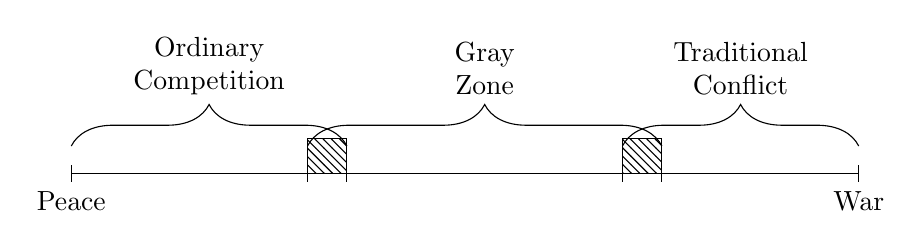
\begin{tikzpicture}
			\draw (0,0) -- (10,0);
			\foreach \x in {0, 3, 3.5, 7, 7.5, 10}
			\draw (\x cm,3pt) -- (\x cm,-3pt);
					
			\draw (0,0) node[below=3pt] {Peace} node[above=3pt] {$ $};
			\draw (1.75,0) node[below=3pt] {$ $} node[above=25pt, align = center] {Ordinary \\ Competition};
			\draw (3,0) node[below=3pt] { } node[above=18pt] { };
			\draw (3.5,0) node[below=3pt] { } node[above=3pt] { };
			\draw (5.25,0) node[below=3pt] {$ $} node[above=25pt, align = center] {Gray \\ Zone};
			\draw (7,0) node[below=3pt] { } node[above=18pt] { };
			\draw (7.5,0) node[below=3pt] { } node[above=3pt] { };
			\draw (8.5,0) node[below=3pt] {$ $} node[above=25pt, align = center] {Traditional \\ Conflict};
			\draw (10,0) node[below=3pt] {War} node[above=3pt] { };
					
			\draw[decorate, decoration = {brace, amplitude = 15pt}, xshift = 0pt, yshift = 10pt] (0, 0) -- (3.5, 0);
			\draw[decorate, decoration = {brace, amplitude = 15pt}, xshift = 0pt, yshift = 10pt] (3, 0) -- (7.5, 0);
			\draw[decorate, decoration = {brace, amplitude = 15pt}, xshift = 0pt, yshift = 10pt] (7, 0) -- (10, 0);
				
			\draw[pattern=north west lines] (3,0) rectangle (3.5,0.45);
			\draw[pattern=north west lines] (7,0) rectangle (7.5,0.45);	
			\end{tikzpicture}
			\caption{Model of Conflict}
		\end{figure}
				
		\citet{schelling_armsinfluence_1966} argues that ``the main consequence of limited war, and potentially a main purpose for engaging in it, is to raise the risk of larger war." Our theory presents a different relationship between, in his terms, limited war and larger war. Instead, a capable actor may choose to engage in limited war to \textit{lower} the risk of larger war. We agree with Powell when he states ``the amount of power the challenger brings to bear affects the stability of the conflict. More specifically, how much power the challenger brings to bear limits how much risk the defender can generate" \citep{powell_nuclearbrinkmanshiplimited_2015}. Where we expand upon his model is in Powell's conceptualization of the military might used by the challenger. Powell defines different values of military might ($p$) as different types or levels of conflict which leads him to the conclusion that the way states fight and the level of violence at which they fight affects the risk of all-out war \citep{powell_nuclearbrinkmanshiplimited_2015}.
				
		A parallel can be made between this analysis of gray zone conflict and the discussion of ``calculated nuclear ambiguity" that surrounded the first Gulf War. Former US Secretary of State James A Baker III described US nuclear policy in the Persian Gulf War as one of calculated ambiguity in reference to the alleged US response to Iraqi use of chemical and biological weapons (CBW) \citep{arkin_calculatedambiguitynuclear_1996}. In 1996, Secretary of Defense Perry said that the US response to Iraqi CBW usage was intentionally ambiguous because the US thought that if Iraq was unsure about what the response to CBW use was, they would be deterred from using them \citep{sagan_casenofirst_2009}. This held true despite a private decision by the White House to not use nuclear weapons in response to a chemical attack, a decision the White House kept secret from the Iraqi government and the Pentagon. The purpose of this ambiguity was the convince the opponent that the worst could happen.
				
		However, calculated ambiguity required a careful line to be toed in being ambiguous. On one hand, President Bill Clinton wanted to avoid falling into the commitment trap that Kennedy faced during the Cuban Missile Crisis where a clear promise about a US response obligated that response because officials felt the US reputation was at stake \citep{sagan_commitmenttrapwhy_2000}. Furthermore, the US did not want to create a visible nuclear option during the Gulf War because of the domestic and international political cost it would face from doing so \citep{arkin_calculatedambiguitynuclear_1996}.
				
		On the other hand, the threat made by the US had to be seen as credible, requiring Clinton to say something. Deterrence is a product of capability and credibility. For deterrence to succeed, the expected cost of punishment multiplied by the probability that the threat will be implemented has to exceed the aggressor's expected gain from initiating a conflict \citep{sagan_commitmenttrapwhy_2000}. What further complicated the Iraqi situation was that the US had forsworn the use of chemical weapons, meaning it could not credibly threaten to response to CBW use in kind. So instead, it opted to escalate with an ambiguous asymmetric nuclear response.
				
		Calculated ambiguity plays an important role in understanding the uniqueness of gray zone conflict because nuclear weapons have forced strategic planners to consider a range of alternative uses of military forces that were not just the upper limit of general nuclear war \citep{stephens_transformationlowintensity_1994}. After World War II, countries wondered how to fight a conventional war in Europe without it escalating to nuclear use. In 1957, Kissinger and Osgood tried to figure out limited war and avoiding escalation by placing restrictions on the types of targets and weapons systems as well as ways to limited the geographic scope of a conflict \citep{woodman_defininglimitedconflict_1991}. In this sense, although gray zone conflict may not be something new, the scope of gray zone conflict may have shifted as a result of historical events. Conflict is certainly a continuum, but we need to do a better of describing where the breaks in that continuum lie. The importance of a new definition of gray zone conflict then is a renewed understanding of the conditions that motivate forms of conflict that lie beneath the break of conventional conflict but above the break of ordinary interstate competition.
				
		Our innovation demonstrates a shortcoming of prior conceptualizations of limited war; the term itself is ambiguous and whether the limited-ness of a war is defined simply by its intensity is unclear. This also helps clarify the relationship between nuclear weapons and limited war. It seems odd to argue that every non-nuclear conflict that a nuclear power engages in should be considered a limited war. When nuclear powers choose to forgo use of their nuclear arsenal, that decision should not be considered gray zone conflict by virtue of its reduced intensity. The level of conflict alone does not determine whether an action should be considered gray zone conflict since that action must be considered in light of its motivation.
				
		But types and levels of conflict are not synonymous, nor should they be grouped together. Our theory expands Powell's by looking at the relationship between \textit{how} states fight and the level of violence at which they are fighting. This can help answer the question of whether or not shifting from one type of conflict to another necessitates an increase in the level of conflict simply because there is a shift. One reason an actor may shift from one type of conflict to another is to shift to a domain where they opponent has a relative weakness. In this case, the attack may not really be increasing the level of conflict on their end, but given defense capabilities that differ by domain for the defender, it could very well be an increase in conflict (the value of $p$) for them. In brief, a change in the type of $p$ by the attack may be interpreted as increasing/decreasing $p$ to different extents and in different directions for the aggressor than the defender.
				
		One metric of intensity is resource allocation and this is where gray zone conflict is important since it can be a strategically calculated decision to under-allocate resources to a conflict (because of deterrence or efficiency) but that has two different outcomes in terms of escalation if the target responds. One could argue that some gray zone activities like cyber are low levels of conflict since they have low levels of resource allocation but they may be seen as escalatory since they are a different type of conflict. As a result, an actor may not realize that one of its actions is gray zone conflict. If a country does not have an appropriate, same-domain, and proportional response to a type of attack then its use may result in the horns of strategic dilemma even if the initiator does not realize it (some argue this is the case with US Prompt Global Strike (PGS)).
				
		Notions of cross-domain deterrence expect gray zone conflict to occur. One important example of this is electronic weapon and cyber attacks that do not directly result in enemy casualties. Russia has the capability to cause deaths with these attacks yet it chooses not to do so. NATO does not quite know how to respond to this because kinetic operations may be too much of an escalation and it may not possess cyber and electronic capabilities that can respond in kind and because attribution may be difficult.
				
	\subsection{Why Gray Zone Conflict Occurs}
		One of the first observations made about gray zone conflict was the uniqueness of its intensity, but the historical examination demonstrates this is not so unique after all. Cases like Russian ``little green men" in Crimea are explained as initiators working around the red lines of their opponents by ``advancing without attacking" to achieve their objectives without using force \citep{altman_advancingattackingstrategic_2017}. The issue then is why are capable actors motivated to pull their punches and engage in gray zone conflict. Thus, the key insight is that gray zone conflict is a choice by actors who are not limited by their means, but may be limited by their ends. Our theory helps explain the strategy and motivation for that action. Here we present two explanations, deterrence and efficiency.

		\subsubsection{Product of Deterrence}
			Gray zone conflict may be the product of prior successes in deterrence. Initiators of gray zone conflict may pull their military punches --- enduring a conflict that is prosecuted in a non-optimal manner from their perspective --- because the alternative risks escalation, such as drawing in additional adversaries that increase the cost of fighting beyond acceptable levels. Initiators in these circumstances are not choosing to fight in the manner they prefer but are instead being deterred from their ``optimal'' mode of conflict. This type of gray zone conflict is thus best thought of as ``war with inhibitions." The initiator's strategy is a compromise between what it does best militarily and what it fears will happen if it adopts its optimal battlefield strategy and tactics. As a result, the initiator cannot expect to perform especially well on the battlefield because their fear of escalation has dissuaded them from implementing their most effective strategy. These actors have risked additional delay, expense, and inconvenience because they have made compromises from what they would do in an unconstrained environment in order to avoid triggering the escalatory responses of targets and target allies.
			
			There are in turn two basic reasons that this might occur (both can exist simultaneously). First, an adversary may possess benefits that would be endangered by escalation to higher conflict intensity or greater conflict scope. Globalization and its associated network of economic interdependencies creates collective incentives to avoid large conflicts that would disrupt commerce. More broadly, changes in the material basis of military and economic power have increased both the incentives and opportunities for ambiguous gray zone aggression in a few important ways. The cost of war has increased because better military technology has made conflict more consequential. Many have argued that deterrence has been a cause of peace but in reality it may be a cause of the absence of high intensity war meaning it leaves open the possibility of gray zone conflict \citep{rauchhaus_evaluatingnuclearpeace_2009}. Peace has also become increasingly beneficial since improvements in communication technology and global trade rely on cooperation in ways that have increased interdependency. Arguably, overt military combat has declined and been replaced with an increase in covert and intelligence operations that have the added benefit of lower body counts. As a result, state interests have been regularized and issues that used to cause war no longer do because globalization has provided forums for peaceful dispute resolution in lieu of war.
			
			While the effects of interdependence on peace are not new, the role of globalization in shaping the type or \textit{intensity} of conflicts, rather than deterring all contests outright seems especially germane to the origins of gray zone warfare \citep{gartzke_measuremeasureconcept_2003, gartzke_complexstructurecommercial_2016}. Traditional conflict comes with a fear of losing out on the benefits of cooperation from ordinary competition. This occurs despite the fact that traditional conflict can often better achieve a nation's objectives than ordinary competition given compromise is less necessary (if it is necessary at all). Since one factor that differentiates gray zone conflict from traditional conflict is the response by the defender, gray zone conflict has an added benefit over traditional conflict in being less likely to trigger a loss of cooperation between those actors. Russia, for example, clearly hoped that incursion into Ukraine would not prevent it from supplying Europe's energy needs, even as Europeans were concerned that their response might endanger access to Russian natural gas. These causes of 21$^{st}$ century peace, in particular increased interdependence, are being exploited by capable actors in ways that subvert deterrence. The benefits to peace provide new ways to hassle target states through gray zone conflict which explains why even though the concept of conflict short of war is not new, the motivations behind it are in ways that warrant updating theories of conflict. This results in the uncomfortable conclusion that the institutional causes of peace in the 21$^{st}$ century may be a cause of gray zone conflict since the fear of losing cooperation creates an incentive to use gray zone conflict over high intensity conflict because gray zone conflict can be initiated without fear of losing the benefits of cooperation.
							
			If interdependence is a ``carrot" encouraging discreet aggression, then deterrence is the ``stick" that makes it costly for an aggressor to go too far. If an initiator has intentionally chosen to limit its engagement, this could represent not a ``new way of war", but instead it is simply an adversary that wishes to avoid triggering escalation. Ukraine is a commonly misunderstood example. Here, the target and/or its allies (Ukraine and NATO) have escalation dominance. Russia knows that were high intensity conflict to occur over Ukraine, it is likely to lose that conflict and thus they are afraid to risk triggering escalation. The risk of triggering a robust NATO reaction arguably mitigated any military logic for a more extensive or overt use of Russian military power in Eastern Ukraine. The fear on both sides of possible NATO involvement arguably led to circumspection in the Russian approach to intervention. When Malaysian Airlines flight MH17 was shot down over Donetsk by a Russian BUK anti-aircraft missile, Moscow was quick to withdraw these and other heavy weapons from the battlefield. Witnessing gray zone conflict here is evidence of deterrence success at higher levels of conflict intensity.
			
			The gray zone thus functions in an area below the threshold created by deterrent threats or economic opportunity. This gray zone has always been there (peace and war have never truly been dichotomous) but that zone has grown as a result of the expanding benefits to peace and increasingly prohibitive cost of war. Competition is bounded by the incentives to cooperate (in the case of interdependence) or at least coordinate (deterrence). Adversaries no longer possess monolithic interests, preferring to compete around the edges, rather than openly thwart the other side in a manner that might maximize military efficiency, but would undermine larger political objectives. Aggression among the interdependent or mutually constrained must be pursued somewhat more furtively, so as not to endanger a broader set of compatible goals.

			One implication of this perspective is that raising the cost of gray zone conflict can cause the initiator to stop without risking escalation. If we are in a world where gray zone strategy has been chosen because of a fear of escalation, then the target making gray zone conflict prone to escalation or retaliatory response should cause the risk-averse initiator to avoid both high and low-level conflict.
		
		\subsubsection{Product of Efficient Warfare}
			If the first explanation for gray zone conflict involves inherent tensions between the use of force and its consequences, the second argument requires no such contrast. Initiators (and their targets) may have decided that pulling one's military punches is, in fact, optimal.  A challenger that is patient and capable relative to its adversaries at low intensities could benefit by choosing a gray zone strategy. Big contests are costly and may not improve one's prospects for victory, especially if a limited contest poses advantages in terms of an initiator's force structure or force posture. While high intensity conflict may accomplish the initiator's goals, it can be perceived as unnecessary overkill if they believe they can accomplish those same goals with reduced effort \citep{altman_advancingattackingstrategic_2017}. Since the 1990s, Russia has had only a limited ability to field and sustain main force units abroad, especially in the face of capable tactical air power.\footnote{As the risk of NATO involvement in Ukraine increased, Russian officials laid heavy hints of their willingness to deploy tactical nuclear weapons. The Russian doctrine of ``escalate to deescalate'' is designed to allow Russia to maintain its conventional advantage against local opponents, while deterring NATO.}  A major upgrade of Ukrainian military capabilities by Western powers would force Russia into a long and costly war of attrition. Better to fight a long and relatively cheap war of attrition, one that Moscow can expect to win. Fighting small can also be advantageous for even a large disputant, if they possess a modest number of highly trained forces.   
			
			It is also important to note that the use of gray zone tactics is generally viewed pessimistically in the West. Gray zone conflict is seen as a dangerous new approach assumed to be available only to adversaries and thus inherently threatening. Gray zone conflict has been described as ``a carefully planned campaign operating in the space between traditional diplomacy and overt military aggression" employed by states with grand geopolitical ambitions \citep{mazarr_masteringgrayzone_2015}. Fear of gray zone conflict has even led some to advocate revamping deterrence to prevent these threats \citep{santoro_healeywrongit_2016, foust_canfancybear_2016, jackson_preventingnuclearwar_2016}. Yet, NATO and U.S. deterrence policy has arguably succeeded in keeping more overt forms of aggression in check. Paying attention to why a challenger has chosen gray zone conflict is not only useful, but it also emphasizes that gray zone strategies are available \textit{to both sides}. A neutral theoretical approach thus implies unexpected advantages in gray zone conflict; the very fact that an adversary is engaging in limited conflict suggests vulnerabilities and opportunities for increased effectiveness on the part of the target and its partners.
	
			This scenario carries the opposite policy implication from the deterrence case. If gray zone conflict was chosen by the initiator because it is a lower-cost means to achieving their goals, then raising the cost of gray zone conflict risks encouraging the initiator to escalate. This may, in fact, be desirable for the target. Assuming that gray zone conflict is not optimal for the target, the target can exploit the escalation effect of inefficient warfare by raising the cost of gray zone conflict, thus preventing the initiator from being able to exploit its low cost means of achieving their goals. In essence, by raising the cost of gray zone conflict, the target and their allies can force the initiator into fighting inefficient warfare.
	
		\subsubsection{Importance of Contrasting Motivations}	
			Understanding why these two possible motivations have contrasting predictions about the consequences of dissuading gray zone conflict requires comparing the options available to the initiator \citep{schram_hassling_2017}. An actor wishing to change the balance of power can do so through ordinary competition, gray zone conflict, or traditional conflict. These strategies all differ in terms of their ability to change the balance of power as well as their costs.
		
			An actor undertakes gray zone conflict when the expected utility of doing so exceeds the expected utility of ordinary competition and traditional conflict. In other words, it's the most preferred choice. Thus, we can infer their preference ordering as being one of two possible options:
		
				\begin{quote}
					\centering
					\begin{tabular}{rcccl}
						Gray zone & $>$ & Ordinary competition & $>$ & High intensity conflict \\
						Gray zone & $>$ & High intensity conflict & $>$ & Ordinary competition
					\end{tabular}
				\end{quote}
		
			These distinct preference orderings explain the importance of understanding the motivation behind gray zone conflict. The former is an example of gray zone conflict motivated by deterrence. The cost of traditional conflict is made sufficiently high by the threat of retaliation so the initiator has compromised and chosen avoided their optimal strategy. The latter is an example of gray zone conflict motivated by efficiency; the initiator would have been willing to go to war to achieve their desired objective, but gray zone conflict represented a way to acquire their objective without incurring unnecessary costs. Russia won't send an entire battalion of tanks to acquire territory in Crimea if it feels a few ``little green men" are sufficient to accomplish that goal.
		
			This point clarifies why raising the cost of gray zone conflict discourages escalation in some cases while possibly encouraging it in others. Raising the cost of gray zone conflict when it is motivated by deterrence discourages escalation since the threat of retaliation invokes the precise costs that the initiator was hoping to avoid in the first place. When motivated by efficiency however, the initiator has already decided that the expected gains from traditional conflict exceed the costs, and thus raising the cost of gray zone conflict simply result in a situation where their more efficient option is no longer efficient, but their objective is still important enough to warrant revisionist measures beyond ordinary competition.
		
		% Add discussion here about equilibriums and how gray zone conflict can be the only non-war equilibrium depending on the preference ordering of states
		
			Gray zone conflict will not always be the optimal choice for an actor. Every conflict happening today should not be considered a gray zone conflict and there is abundant evidence that ordinary competition continues to characterize most state interactions. If a capable state hopes to change the balance of power on the cheap and without triggering a reaction, then initiating gray zone conflict is a reasonable strategy. However, if an actor hopes to coerce another into changing its behavior, then gray zone conflict is less strategic. The appeal of gray zone conflict is the ability to challenge the balance of power while limiting the reaction of the target. Thus, foreign policy goals that are driven by coercion will not be best achieved by gray zone conflict. Rather, it is a tool best left to those hoping to shift the balance of power via attrition.

\section{Empirical Evidence}
	To test our theory that gray zone conflict is a policy choice by capable actors motivated by either the target's successful deterrence or the possibility of more efficiently achieving one's objectives, this paper employs a comparative case study method focused on Russian cyber attacks on NATO countries. We employ a most similar case comparison by choosing cases that have the same gray zone conflict initiator (Russia), the same target (the West), and the same means (cyber attacks), but that differ in what motivated Russia to choose gray zone conflict over another ordinary competition or high intensity conflict \citep{bennett_casestudymethods_2007}.
		
	One of the primary ways differences in motivation can be inferred is the result of the NATO response. Our theory predicts that when gray zone conflict is chosen because of successful deterrence, responding to gray zone conflict will de-escalate the situation and result in the initiator choosing ordinary competition as their next preferred option. When gray zone conflict is chosen because it's the most efficient means of achieving their objective, responding to gray zone conflict will escalate the situation because the initiator now has to resort to more costly high intensity conflict to achieve their objective. We test our theory against two alternative explanations. First, that Russia's decision to use cyber attacks as a form of gray zone conflict is a function of the duration of the conflict and second that cyber attacks are more likely to be employed in more recent conflicts as a result of technological advancements.

	\begin{quote}
	\begin{table}[H]
	\caption{Russian Interventions}
	\label{fig_losg}
	\begin{adjustbox}{width=1.2\textwidth,center=\textwidth}
		\begin{tabular}{|l|l|cccccc|}
			\hline
			 & & \textbf{Chechnya} & \textbf{Georgia} & \textbf{Ukraine} & \textbf{Estonia} & \textbf{Kosovo} & \textbf{US} \\
			\hline
			\multirow{4}{*}{\textbf{Deterrent Gradient}}
			& Distance from DC & 6 & 5 & 4 & 3 & 2 & 1 \\
			& NATO & - & - & - & Y & (Y) & Y \\
			& Russia Military Advantage & Y & Y & Y & Y & (-) & \\
			& Russia Vital Interest & Y & Y & Y & (-) &  &  \\
			\hline
			\multirow{4}{*}{\textbf{Behavioral Response}}
			& Military Intervention & Y & Y & (Y) &  &  &  \\
			& Paramilitary/Covert Ops & Y & Y & Y & (Y) &  &  \\
			& Cyber Disruption & Y & Y & Y & Y & Y &  \\
			& Information Ops & Y & Y & Y & Y & Y & Y \\
			\hline
			\multirow{3}{*}{\textbf{Theories}}
			& (E)fficiency vs (D)eterrence & E & D/E & D & D & D & E \\
			& Duration (S/M/L) & L & S/M & L & S & S & S/M \\
			& Maturation (Chronological) & 1 & 4 & 5 & 3 & 2 & 6 \\
			\hline
		\end{tabular}
	\end{adjustbox}
	\end{table}
	\end{quote}

	Table \ref{fig_losg} shows the role that deterrence plays in motivating gray zone conflict by Russia. This represents 4 important and known Russian cyber attacks against the West (Georgia, Estonia, Ukraine, and the United States) as well as two other cases (Chechnya and Kosovo) to serve as a benchmark. In each case, we seek to explain whether Russia pulled its punches by engaging in cyber warfare because of deterrence or because of efficiency. For each case, we code 4 factors that influence the degree of deterrence affecting Russia's decision of how to initiate conflict (deterrent gradient), Russia's behavioral response indicates the means deployed in that conflict (behavioral response), and then compares the expectations of our deterrence-motivated theory with the two alternate explanations described earlier (theories). For the deterrence gradient, we use ``distance from DC" as a proxy for Russian interests and how easy it is for the West to get forces to that area to counter Russian activities. ``NATO" demonstrates whether or not the geographic target of Russian intervention is a NATO member and whether it is expected that NATO will come to the aid of the country in question. We expected that interventions where a NATO response is anticipated or likely will be cases where Russia undertakes gray zone conflict because of the effect of general deterrence. This factor thus best captures the role of proxies/allies on the part of the target country. Russia intervention in Estonia, for example, took into account the military capabilities of NATO writ large and the likely response Russia would face from Estonian allies like the United States. The geographic target of Russia intervention should thus not be confused as synonymous with the political target of the Russia intervention and the actor whose deterrence capabilities are being considered because of the role of allies. The last two factors code whether Russia has a conventional military advantage over the geographic target and whether it has vital interests that are at stake in that country. The behavioral response parameters are self-explanatory and describe the combination of actions Russia undertook during their military intervention. The table indicates whether our theory argues that Russia's strategy was driven by efficiency or deterrence and also codes the duration of each intervention as well as ordering them temporally. The latter two factors demonstrate that neither of those two theories explain the pattern of Russian cyber operations as well as our theory.

	\subsection{Georgia}
		In early 2008, an election was held in Georgia following accusations that the incumbent, President Mikheil Saakashvili, was suppressing political dissidents. Despite the accusations, he was re-elected in part due to his promise to uphold Georgian territorial integrity. At this same time, Georgia also declared their aspiration to join NATO which was welcomed by NATO at the Bucharest Summit Declaration. Soon after, suspicion arose within the Georgian government that Russia was responsible for a wave of cyberattacks against Mikheil Saakashvili that included DDoS attacks, ICMP floods, TCP SYN floods, and HTTP floods \citep{shakarian_2008russiancyber_2011}. The Shadowserver Foundation, a group that tracks cyber attacks, traced these attacks back to a Machbot controller that had over 15,000 bots issuing these attacks \citep{nazario_btf8indepthlook_2008}. These attacks continued for months and targeted internet connections that were connected to physical infrastructure like oil pipelines. This was the first time that known cyberattacks had coincided with a kinetic shooting war given the Russian invasion into Georgia.
		
		This combination of cyber influence and disruption (propaganda, espionage, DDoS), active measures (covert military operations), as well as norms violations and sovereignty infringements (e.g. ``passportization", airspace incursions) is characteristic of gray zone conflict calculated to achieve political and security objectives without triggering overt military conflict. Recourse to conventional military and legal tools was foreclosed to Georgia and its allies, because the challenge of attribution for cyber operations provided the suspected perpetrators with plausible deniability. Other low intensity activities were calibrated to avoid thresholds justifying armed self-defense.
		
		We argue here that Russian cyberattacks against Georgia in 2008 is an example of gray zone conflict initially motivated by deterrence success but later motivated by efficiency. Deepening US and NATO interests in post-revolutionary Georgia likely led Russian leadership to pursue gray zone conflict as an optimal strategy for altering the status quo of frozen conflicts in Russia’s near abroad, despite enjoying escalation dominance over the defending state, Georgia. Congruence between the Kremlin’s irredentist policies  and secessionist attitudes in Abkhazia and South Ossetia stoked pro-Russian sentiment in restive regions inside Georgian territory, producing negative synergies that intensified in the Summer of 2008 that rose above ordinary levels of interstate competition \citep{medvedevvowsprotect_2008, deibert_cyclonescyberspaceinformation_2012}. One explanation for this could be that American investment in modernizing the Georgian military had raised the cost of engaging in conventional warfare. Conventional military deployment might have been the more efficient option for resolving conflict in Russia’s favor, particularly given the effectiveness of information interdiction and crippling of Georgian communication infrastructure prior to hostilities, but US and NATO support for the Georgian government may have been perceived to be strong enough that there was at least a chance that Georgian allies would be drawn into conflict. Alliance maintenance, issue slippage, and ideational affiliation were forces that bound allies to a weak state under threat. Deterrence was operational until Georgia miscalculated the extent of that deterrence which is what triggered a Russian invasion. Russia realized it could invade with a freehand.

	\subsection{Estonia}
		The familiar 2007 case from Estonia reflects a cautious Russian effort in the gray zone constrained by general NATO deterrence. The retributive cyber rioting that took place after a Soviet-era statue was relocated from the center of Tallinn to its outskirts temporarily altered the status quo in Russia’s favor without eliciting punishment. All sides – belligerents, their agents, and the targets – were relatively inexperienced with cyber operations at scale in 2007. The combination of immature organizational processes for dealing with hostile cyber operations, risk of over-reaction by the recipient state, or its allies, could have led to miscalculation, and unintended escalation into the conventional warfighting domains, where NATO maintained escalation dominance \citep{slayton_whatcyberoffensedefense_2017}. These risks and the cross-domain threats arrayed against Russia likely motivated the choice to engage by limited means.
		
		Though sometimes cast as a Russian victory, the Estonia event was highly visible, and galvanized states to begin thinking through the implications of operational cyberspace. As Western governments and alliances began hardening networks against vulnerabilities exposed by the crippling Internet traffic directed into Estonia, it appears that the space for effective ad hoc gray zone cyber operations narrowed. Policy actions and the establishment of new institutions raised the profile and resources of cyber defense capability, eliminating some of Russia’s leverage over its neighbor. NATO’s network resiliency built up since 2007 through a combination of technical defense and efforts to overhaul member states' defenses, provide training, and deploy rapid network repair teams confers deterrent reputational effects on the alliance. \citet{lindsay_coercioncyberspacestabilityinstability_2017} point out that, ``skilled cyber defense, above and beyond the ability simply to detect threats, enhances deterrence by denial." As a consequence, cyber operations from 2007 onward exhibit more planning; the potency of more mature cyber toolkits was proven just a year later in Georgia.
	
	\subsection{US Election}

\section{Discussion}
	An important implication is thus that gray zone challenges are an inevitable consequence of establishing deterrence. If deterrence is to keep up with these challenges, it must continue to adapt as well. In a sense, deterrence is little more than a strategy to buy time against an adversary that is strongly committed to changing the status quo \citep{george_deterrenceforeignpolicy_1989}.
		
	While not discussed in the context of gray zone conflict, George and Smoke did discuss the notion of ``designing around" deterrence as an action taken by adversaries in response to deterrence \citep{george_deterrenceamericanforeign_1974}. Here, adversaries consider the options available for challenge deterrence and they identify the option that ``offers an opportunity for gain while minimizing the risk of an unwanted response by the defender" \citep{george_deterrenceforeignpolicy_1989}. However, George and Smoke describe this as a deterrence failure, an argument that gained empirical traction in analysis of the 1973 war where Egypt ``designed around" Israel's deterrent capability \citep{stein_calculationmiscalculationconventional_1989}. Our perspective, by comparison, is that ``designing around" deterrence through the initiation of gray zone conflict is a sign of deterrence success.
		
	Some, however, have viewed this as a deterrence success. \citet{lieberman_reconceptualizingdeterrencenudging_2012} argues that ``designing around" is a sign of successful deterrence because an adversary has limited their challenge as a result of the perceived response from the defender. This demonstrates that there is nothing necessarily new about gray zone conflict, and scholars have long recognized it as a problem. The fact that it seems new now is a testament to ignorance of historical parallels, failure by scholars to address the problem, and possible something interestingly different about recent challenges. Part of that difference could be an evolution in what type of deterrence gray zone conflict is ``designing around." While previous actions by adversaries were designed around \textit{immediate} deterrence, gray zone conflict may represent cases of adversaries challenging \textit{general} deterrence. The value of our model of conflict is identifying the types of moves available to an initiator given the constraints of successful general deterrence and explaining why that results in gray zone conflict as opposed to ordinary competition or traditional conflict as it did before.
		
	One purpose of gray zone conflict is to dominate the OODA loop (observe, orient, decide, and act) by paralyzing your opponent because they don't know how to react to a novel lower level of escalation in a space opened up by the causes of peace which is the argument made with the horns of the strategic dilemma \citep{maxwell_grayzonesubject_2016}. One possible result of this is that if an actor like Russia feels even more threatened by NATO, it may be willing to deploy even grayer zones of conflict as a response to successful deterrence.
		
	Our theory's new clarification about the distinction between gray zone conflict and asymmetric warfare by less capable actors also matters for US foreign policy strategy. Observationally, `limited wars' often look similar. Limited actions by Russia in Crimea use similar forces and are of a similar scope to actions undertaken by non-state actors. But although the behavior looks the same, the motivations are different. In one case, an adversary's actions are limited by choice while in the other case an adversary's are limited by necessity. Failure to appreciate this distinction results in the ill-advised application of counter-terrorism or asymmetric warfare doctrine and strategy to cases of gray zone conflict with potentially disastrous implications.
	
	The examples provided of Russian gray zone operations carried out as cyber attacks in Ukraine, Georgia, Estonia, and the US election have shown the role that deterrence has played in motivating Russia's strategic decisions. Deterrence manifested itself via geographic proximity to the US, NATO membership of the target country, whether Russia had military superiority relative to the target in question, and whether that conflict zone represented a vital interest for Russia. The cases where Russia was least deterred, as measured by these four operationalizations, were those where Russian operations were most characterized by gray zone conflict.

	Although not discussed in detail here, Russian operations in Chechnya and Kosovo also provide useful context. Russia’s misjudgement about the intensity of military resistance against its effort to reclaim Chechnya was mirrored in the cyber domain. Chechen loyalists repeatedly thwarted Russian strategic planners’ effort to control the information environment by launching attacks against Russian state media, and re-launching or relocating websites with content that competed with Russian portrayals of the war \citep{bullough_russianswagecyber_2002}. The Chechen insurgency and online ingenuity no doubt raised costs for Russia, but cyber operations were not pivotal because they operated as an adjunct to covert and conventional military operations. Russia judged intervention to be the most efficient way to prosecute war in Chechnya, and eventually prevailed; disinformation and disruption propagated in the cyber domain were not decisive. But Chechnya and Kosovo are significant cases in the history of Russian cyber campaigns for occurring at a time when Russia appeared to be testing a new conceptualization of cyber-enabled conflict requiring \textit{fewer elements} of power to achieve political-security objectives, the defining feature of gray zone conflict \citep{bullough_russianswagecyber_2002}.
		
	The targeting of websites sympathetic to Chechnya, and defacement of NATO websites during the intervention in Kosovo, appear to fulfill a vision of contemporary conflict taking shape around the time Vladimir Putin ascended the Russian presidency. In late 1999, deputy chief of the Russian Security Council, Vladimir Vasilyev pronounced, ``[i]t is clear that today a fight is going on over public opinion both inside the country and abroad, and that whoever gets to shape it, to direct it, is going to be winning in this process" \citep{broadcastingreview1999_1999}. In 2001, while Putin defended Russia’s policy in Chechnya during a special Internet interview live streamed by the BBC his spokesman explained, ``We wanted to show that we understand that the Internet is an important part of forming public opinion" \citep{tyler_talkativeputindemonstrates_2001}. If the dividends of capturing public opinion match those gained from capturing territory and come at much lower cost, then it would be optimal for an initiator to advance political objectives by operating primarily in the gray zone \citep{snegovaya_putininformationwarfare_2015}. Becoming proficient in gray zone operations, an initiator could alter the status quo without waging war, and foreclose target state justifications for responding with conventional deterrence measures \citep{lin_operationaldoctrinehybrid_2015}.
	
\section{Conclusion}
	This paper argues that while ``conflict short of war" is an old concept, gray zone conflict requires a new understanding that focuses on explaining its causes. In particular, this paper introduces the concept that gray zone conflict is conflict involving capable actors who intentionally limited the intensity and capacity that they dedicate to fighting because they both prefer low-intensity to high-intensity conflict. The gray zone of the spectrum of conflict is expanding because of new causes of peace in the 21$^{st}$ century --- namely the ``carrot" of interdependence and the ``stick" of deterrence. An actor's motivation for choosing to operate in the gray zone area of that spectrum determines the outcome of the target's response.
	
	We offer a re-conceptualization of gray zone conflict through the lens of deterrence. Understanding a nation's motivation for engaging in gray zone conflict enables the target to determine its best response. A challenger that initiates gray zone conflict has made a calculation about the type and degree of provocation that would trigger an escalatory response from the defender. Our theory notes that the risk of high level conflict may fail to disincentivize, and may even facilitate, low level conflict \citep{snyder_balancepowerbalance_1967}. Gray zone strategies have developed as a response to the success of ``high stakes" deterrence, as an end run around their (effective) restrictions. ``Low stakes" gray zone conflict emerged as actors dialed back the level of violence to minimize exactly the risks posed by classical deterrence in practice. The high benefits of peace made possible by interdependence and deterrence have created a platform for adversaries to be revisionist and hassle without triggering a loss of cooperation.
	
	It is critical for decision makers to know why the initiator chose limited gray zone conflict because that changes the implication of raising the cost of gray zone conflict. If we are in the first situation where the initiator chose gray zone because they are cost-averse, then raising the cost of gray zone conflict will likely result in peace. However, if we are in the second situation where the initiator chose gray zone conflict because they prefer limited war as a lower-cost means of achieving their objectives, then raising the cost of gray zone conflict could risk escalation. The classic debate in security studies between the deterrence model and the spiral model applies to gray zone conflict in a novel way. Whether the response to gray zone conflict inhibits conflict (deterrence model) or inflames conflict (spiral model) depends on whether the initiator's actions are influenced and motivated by previous rounds of deterrence success.

\bibliographystyle{apsr}
\bibliography{grayzone_bib}

\end{document}